\documentclass{tufte-book}

\usepackage{graphicx}
\setkeys{Gin}{width=\linewidth,totalheight=\textheight,keepaspectratio}
\graphicspath{{graphics/}}

\usepackage{xcolor}

\usepackage{listings}
\lstset{
	basicstyle=\ttfamily,
	breaklines=true,
	xleftmargin = 0.5cm,
	framexleftmargin = 1em
}

\title{Delve into ESP32}
\author{Henrik Samuelsson}

\begin{document}
	\maketitle
	
	\cleardoublepage
	\chapter*{Development Setup}
	
	This chapter discusses hardware and software needed to be able to do the exercises and projects presented in this book. The best way to learn is by experimenting and trying real things by yourself as opposed to just reading theoretical background material or watching videos.
	
	A number of different components are required to complete all the projects presented in this book. If your budget is limited so will you be  able to do many of the projects with just a handful of components, and each one is not really expensive either.
	
	\section{Mandatory Hardware}\label{sec:hardware}
	The following things is a must if you really want to become familiar with the ESP32.
	
	\begin{itemize}
		\item Computer for development of software to be run on a ESP32
		\item ESP32 development kit
		\item Bread board
		\item A basic selection of passive and active electronic components
	\end{itemize}
	
	Each type of needed item is discussed more in detail in the following sections.
	
	\subsection{Development Computer}
	A computer running Linux, Windows or macOS is needed to build the software to be run on the ESP32. The bulk of the projects in this book have been developed and tested on a computer running Ubuntu 16.04, so this is the preferred operating system. Most things should work under other operating system but the ride might not be as smooth.
	
	Hardware specs on the computer are really not high. Computer to be used should have one or two free USB ports. There must also be some free disk space for software development tools. Other than that so should pretty much anything work.
	
	\subsection{ESP32 Development Kit}
	A development board with an ESP32-WROOM module is considered mandatory to be able to test the programs that you will create. Espressif, the company behind the ESP32, have released a development board named ESP32-DevKitC that can be bought for about \$15. Do a web search and you should find several vendors that sell it on for example eBay or Amazon. It could also be so that your own favorite electronic components vendor have it in stock.
	
	There are also various variants of the official development board developed by third parties. The cheapest ones can primarily be found on Chinese on-line market places. This can be a way to save a little money but there will usually be a few weeks of waiting for the order to arrive if yoxleftmargin=.25in,u do not live China.
	
	An USB cable is needed to connect the development board and your computer. Exact cable needed depends on the computer and what development board being used. USB A to micro USB is probably the type that you need. Check the ports of your computer and the connector on the development kit before buying.
	
	\subsection{Bread Board}
	Many of the projects requires various electronic components to be connected together. A fast way to hook up components is by using so called bread boards. Bread board comes in various colors and sizes see below picture for an example of a board with 830 connection points.
	
	\begin{figure}
		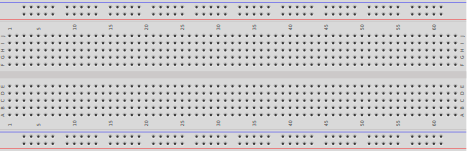
\includegraphics{bread_board.png}
		\caption[Bread board $n$.][6pt]{A common type of bread board. There are plenty of connections points and rails for dual supply voltage.}
		\label{fig:bread_board}
	\end{figure}
	
	The ESP32-DevKitC is bread board friendly and can be plugged in to the bread board directly. But it is fairly wide and will cover many connection points that we will want to have free to be able to connect other things. The solution is to have multiple boards connected together by the same principle used as when laying a jigsaw puzzle. Notice the three small knobs on the bottom of the board in the picture these will fit holes located at backside of the the top of the board. The board you want to have should be of this type that can be connected together with other boards. So search for a ''830 bread board`` that is specified to be able to be connected together and buy two of these boards. An alternative is to search for ''1660 bread board`` and you will get hits were two bread boards are already mounted together for you on a metal plate. Choose either one of these two options but make sure that the bread boards have gotten good reviews by other users because there are a lot of products out there that works less well. 
	
	\subsection{Electronic Components}
	A basic supply of electronic components will be needed for the projects. The components can be bought as separate units but it is easier and usually cheaper to buy a complete kit. There are starter kits, sufficient for our	columns=fullflexible, needs, that can be bought for around \$15. These kits can be found at the same places where you buy your ESP32 development kit. Search for ``Arduino starter kit'' or ``bread board starter kit''. Note that the the kit does not need to contain an actual Arduino micro controller, the ESP32 will play the role as the controller in our projects.
	
	The following list summarizes some of the components that should be included in your collection of electronic components.
	
	\begin{itemize}
		\item Jumper wires
		\item Dupont wires
		\item An assortment of different resistors
		\item Some different ceramic and electrolytic capacitors
		\item Push buttons
		\item LED's in some different colors 
		\item Potentiometer
	\end{itemize}
	
	\section{Software}\label{sec:software}
	
	The process of getting the ESP32 to run our own software depends on the steps and building blocks illustrated in figure~\ref{fig:software_anatomy}.
	
	The very basic foundation of our software will be some packages that we must have on our development computer. On top op these packages so is there a library of ESP32 specific code provided by Espressif. This library is called Espressif Internet of Things Development Framework (ESP-IDF). This library abstracts away some of the hardware specific details and speeds up the development. The final piece of code that can be seen in figure~\ref{fig:software_anatomy} is labeled Our code and this will be project specific code written by us to make the ESP32 do what we want it to do.
	
	When we are done writing a part of our code and shall test it so will we first build a binary file, this is done by running programs and scripts from a set of tools refereed to as the tool chain. A binary file will be the result of an successful build. This binary shall finally be download to a ESP32 and if we have written to code correctly so will the ESP32 start executing the code and start to behave as we intended. 
	
	\begin{figure}
		\includegraphics{software_anatomy.png}
		\caption[Software development $n$.][6pt]{Overview of the software blocks and steps needed to get an application running on the ESP32.}
		\label{fig:software_anatomy}
	\end{figure}
	
	\subsection{Software Installation}
	Exact way to install the software needed to be able to build for the ESP32 depends on what operating system your development computer is running.
	Only installation instructions for Ubuntu Linux is provided here. Instructions for other operating systems can be found by searching on-line for ''Espressif ESP32 installations instructions``.
	
	\subsection{Get Software Packages}
	First make sure that all needed packages are available by opening a terminal window and execute the following command. There shall not be any line breaks in the command. The line breaks seen below are just there to be able to fit the command on the page.
	
	\begin{lstlisting}
sudo apt-get install git wget make libncurses5-dev flex bison gperf python python-serial
	\end{lstlisting}
	

	 
	
\end{document} 